\documentclass[a4j,uplatex,dvipdfmx]{jsarticle}
\usepackage{amsmath}
\usepackage[dvipdfmx]{graphicx}
\usepackage{tcolorbox}
\tcbuselibrary{breakable, skins, theorems}

\title{確率情報理論第7回 解答}
\author{加藤まる}
\date{2020/03/07}

\begin{document}
\maketitle
\bf キーワード:
\rm

\section*{本日の問題解答}
確率変数$X$が正規分布$N(0,1)$に従うとき、確率$P(|X|\ge2)$について。
\begin{itemize}
  \item[(1)] 標準正規分布表から真の値を求めよ\\
    標準正規分布表より、$x=2.0$では0.0228であるから、$0.0228\times 2=0.0456$が真の値である。\\
    (2倍する理由は解説に書いています。)
  \item[(2)] チェビシェフの不等式による上からの評価値と比較せよ。(値はかなり異なる) \\
   チェビシェフの不等式より、
   \begin{equation}
     \begin{split}
      P(|X-m|\ge k \sigma) &= P(|X-0|\ge k \times 1) \\
      &= P(|X| \ge k)
     \end{split}
   \end{equation}
   よって、与式より$k=2$である。
   \begin{equation}
     \begin{split}
      P(|X| \ge 2) &\le \frac{1}{k^2} \\
      &= \frac{1}{2^2} = \frac{1}{4}
     \end{split}
   \end{equation}
   以上より、上からの評価値は$\frac{1}{4} = 0.25$であり、真の値である0.0456よりかなり大きい。
    
\end{itemize}

\section*{本日の問題解説}
\begin{tcolorbox}[
  title = チェビシェフの不等式,
]
確率変数Xが平均値$\mu$と分散$\sigma ^2$となるとき,任意の正数kについて次が成り立つ。
  \begin{center}
    $\displaystyle P(|X-\mu|\ge k)\le \frac{\sigma ^2}{k^2}$
  \end{center}
  \end{tcolorbox}

\begin{tcolorbox}[
    title = 標準正規分布表,
  ]
  「標準正規分布に従うZがとる値がz以上となる確率$P(X\ge z$」を求められる。\\
  \begin{center}
    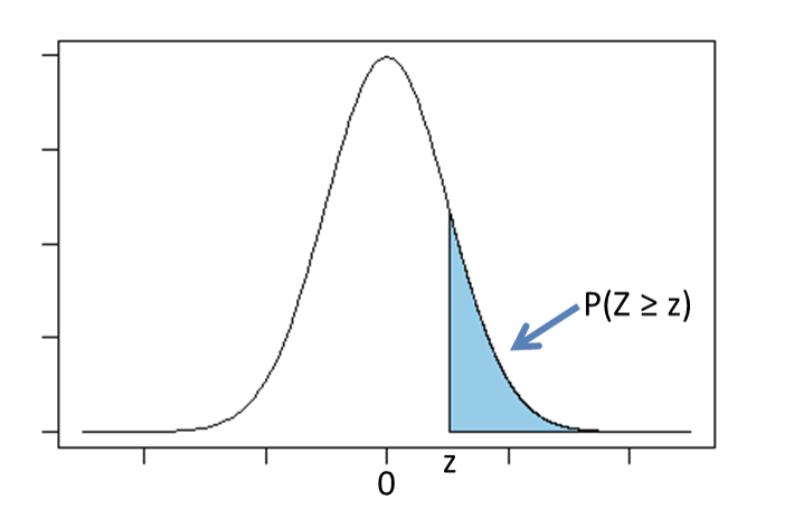
\includegraphics[width=10cm]{ans07_02.png}\\
  \end{center}
  出典:統計WEB(https://bellcurve.jp/statistics/course/7805.html) 
    \end{tcolorbox}

標準正規分布表で求められるのは片側だけ(図の青い部分)だが、チェビシェフの定理で考えているのは絶対値つきで両側を考えている。
そこで、標準正規分布は真ん中で対称的であることから2倍することで$P(|X|\ge z)$の確率の真の値を求めている。
\\ \\ 
(1)で求めた真の値と、(2)で求めたチェビシェフの不等式での上からの評価値は大きく違っている。チェビシェフの不等式では少し
大きな評価になっていることは知識程度に覚えておくとよいかも(私的意見)。
\\
\section*{おかわり問題解答}
確率変数$X$が
\begin{equation}
  f(x)=
 \begin{cases}
   x+1~~~(-1\le x<0)\\
   1-x~~~(0\le x<1)\\
   0~~~~~(otherwise)\\
 \end{cases}
\end{equation}
に従う場合を考える。
\begin{itemize}
  \item[(1)] 期待値を求めよ。
   \begin{equation}
     \begin{split}
       E[X] &= \int_{-\infty}^{\infty} x f(x) dx\\
       &= \int_{-\infty}^{-1} x\times 0\ dx + \int_{-1}^{0} x(x+1)\ dx + \int_{0}^{1} x(1-x)\ dx + \int_{1}^{\infty} x \times 0\ dx \\
       &= 0
     \end{split}
   \end{equation}
  \item[(2)] 分散を求めよ。
  \begin{equation}
    \begin{split}
      V[X] &= \int_{-\infty}^{\infty} (x-E[X])^2f(x) dx \\
      &=\int_{-\infty}^{-1} x^2\times 0\ dx + \int_{-1}^{0} x^2(x+1) dx + \int_{0}^{1} x^2(1-x)\ dx + \int_{1}^{\infty} x^2 \times 0\ dx \\
      &=\frac{1}{6}
    \end{split}
  \end{equation} 
  \item[(3)] $\displaystyle P(|X|>\frac{1}{4})$となる確率をチェビシェフの不等式から求めよ。\\
  チェビシェフの不等式は
  \begin{equation}
      P(|X-\mu|>k)\ge \frac{\sigma ^2}{k^2}
  \end{equation} 
  である。よって、
  \begin{equation}
    P(|X|>k)\ge \frac{\frac{1}{6}}{\left( \frac{1}{2} \right)^2} = \frac{2}{3}
  \end{equation}
\end{itemize}

\end{document}